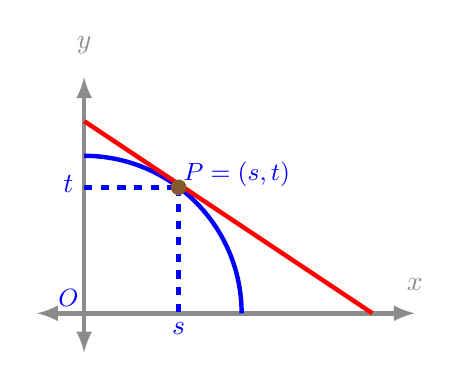
\begin{tikzpicture}[scale=2,
         dot/.style = {
     fill = black!30!brown,
      circle,
      inner sep =2pt,
      minimum size = 4pt
    }
  ]
%%%%%%%%%%%%%%%%%%%%%%%%%%%%%%%%%%%%%%
 %\draw [very thin, style=gray!50, step=0.5] (-3,-2) grid (3,2);
 %\draw [thin, gray!60] (0,0) grid (9,9);
\coordinate (O) at (0,0);
\coordinate (Y) at (0,1.5);
\coordinate (X) at (2.1,0);
\coordinate (X1) at (-0.3,0);
\coordinate (Y1) at (0,-0.25);
\coordinate (D) at (0.6,0);
\coordinate (E) at (-0.6,-0.8);
\coordinate (P) at (0.6,0.8);
\coordinate (C) at (0,0.8);
\coordinate (E) at (-0.6,-0.5);
\coordinate (F) at (1,0);
\coordinate (A) at (0,1.22);
\coordinate (B) at (1.83,0);
\coordinate (G) at (0.87,0);
\draw[color=gray!90,ultra thick,latex-latex]           (X1)node[
                               label = {}]{}-- (X) node[
                               label = {above:$x$}] {};
\draw[color=gray!90,ultra thick,latex-latex]           (Y1)node[
                               label = {}]{}-- (Y) node[
                               label = {above:$y$}] {};
%\draw[blue,ultra thick] (O) circle [radius=1cm];
\draw[blue,ultra thick] (1,0) arc (0:90:1); 
\draw[color=blue,ultra thick,dashed]           (P)node[
                               label = {}]{}-- (D) node[
                                label = {}] {};
\draw[color=red,ultra thick]           (A)node[
                               label = {}] {} -- (B) node[
                                 ] {};
\draw[color=blue,ultra thick,dashed]           (C)-- (P) node[dot, label = {}
                             ] {};
% \draw[color=red,ultra thick]           (C)node[
 \draw[color=blue] (-0.1,0.1) node {\small $O$};
 \draw[color=blue] (-0.1,0.82) node {$t$};
\draw[color=blue] (0.97,0.88) node {\small $P=(s,t)$};
\draw[color=blue] (0.6,-0.1) node {$s$};
  \end{tikzpicture}
